

%  while true ; do rsync /home/imaseki/OneDrive/C105/C105Fig/* ./C105Fig/color/ ; python3 ./python/convert_gray_scale.py --input-dir ./C105Fig/color --output-dir ./C105Fig/gray  ; sleep 30 ; done

% 画像の配置は最後に再度確認する

% 推敲TODO
% 節タイトルはパワポ感覚でつけていきたい。


\documentclass[a5paper,twoside,dvipdfmx]{jsarticle}
\AtBeginDvi{\special{pdf:mapfile haranoaji.map}}
\usepackage[dvipdfmx]{graphicx}
\title{実践PEFT

~ご家庭のGPUでLLM fine-tuning~}
%\author{お椀の底の玉}
\date{}

\usepackage{ascmac}

\usepackage{caption}
\captionsetup[table]{font={scriptsize}}

\usepackage{mathtools}
\mathtoolsset{showonlyrefs=true}

\usepackage[top=30truemm,bottom=20truemm,left=25truemm,right=25truemm,headsep=5truemm]{geometry}

\usepackage{url}

\usepackage{color}

\usepackage{type1cm}

\usepackage{bxpapersize}

\usepackage{booktabs}

\usepackage{listings,jlisting} %日本語のコメントアウトをする場合jlistingが必要
%ここからソースコードの表示に関する設定
\lstset{
  language=Python,
  basicstyle={\ttfamily},
  identifierstyle={\small},
%  commentstyle={\smallitshape},
  keywordstyle={\small\bfseries},
  ndkeywordstyle={\small},
  stringstyle={\small\ttfamily},
  frame={tb},
  breaklines=true,
  columns=[l]{fullflexible},
  numbers=left,
  xrightmargin=0zw,
  xleftmargin=0zw,
  numberstyle={\scriptsize},
  stepnumber=1,
  numbersep=1zw,
  lineskip=-0.5ex,
  showstringspaces=\false
}

\pagestyle{empty}

\usepackage{fancyhdr}  
\pagestyle{fancy}
\fancyhead[RO,LE]{\thepage}
\fancyhead[RE,LO]{\nouppercase{\leftmark}}
\fancyheadoffset[R,L]{1cm}
\cfoot{ }


\usepackage{jumoline}
\setlength{\UnderlineDepth}{3pt}

\begin{document}

% \mcfamily	

\tableofcontents

\newpage

\maketitle

\fontsize{9pt}{16pt}\selectfont

\section{はじめに}

\subsection{本書の目的}

ChatGPTが登場してから2年、Large Language Model (\textsf{LLM})は世界を席巻しバズワードの代表格となりました。今やAIによるちょっとした推論なら、プログラムを書かずとも自然文で命令するだけで簡単に実行できます。プロンプトエンジニアリング時代の到来です。

しかしだからと言って機械学習が不要になったわけではありません。プロンプトエンジニアリングで達成できる性能は限定的であり、教師データを用いて直接モデルの重みパラメータを最適化する\textsf{fine-tuning}の方がより高い精度を狙えます。またプロンプトエンジニアリングはモデルが変わると最適なプロンプトも変わってくるため再度プロンプトをチューニングする必要がある一方で、fine-tuningであれば学習を実行するためのデータとプログラムは同じものを使いまわすことができます。


一方でLLMは非常に巨大なため、個人のGPUでfine-tuningを行うのは困難です。例えばGPT-3.5のパラメータ数は約3550億で\footnote{なおGPT-4のパラメータ数は非公開です。}、これを全て32bitの浮動小数点数(float)で扱おうとするとモデルをメモリに載せるだけで1.4TBも必要になります。これに対し個人で購入できるGPUのメモリは比較的購入しやすいもので8GB~12GB、業務用に片足を突っ込んだ価格のハイエンドモデルであるNVIDIAのGeforce RTX 4090でも24GBしかありません。さすがにこれでは学習どころか推論もままならないため、この本でも取り扱いはしません。

一回りパラメータ数が小さいGPT-2ならどうでしょうか? こちらはパラメータ数15億で、32bit floatなら6GBで収まります。これならfine-tuningもできる……とはいきません。推論時と異なり、学習時にはモデル自体が必要とするメモリと同じだけ、\textsf{勾配}と呼ばれるパラメータ更新の差分を管理するためのメモリも用意しなければなりません。つまり6GB $\times$ 2 = 12GBが必要です。fine-tuningの手法によっては勾配に加えてそのモーメントもモデルのサイズ分、またはこの2倍保持しておく必要があり、これも含めると最大で6GB $\times$ 4 = 24GBも要求します。さらには学習中に行われる勾配順伝播・逆伝播の計算にもGPUメモリは必要となり、庶民的なGPUでは動かすのは厳しいです。

またメモリにどうにか載せたとしても、LLMのfine-tuningは精度を出すのが難しいです。事前学習済みなので一から学習するよりはデータが少なくて済むものの、パラメータ数が大きい分fine-tuningにも大量のデータが必要になるでしょう。

これらの問題を一挙に解決するのが、本書の主題であるParameter Efficient Fine Tuning (\textsf{PEFT})です。PEFTはLLMのパラメータを固定したままfine-tuningします。どういうことかというと、LLMの入力であったりレイヤーの間であったりに追加で少数の学習可能な重みを含む計算を挿入し、これだけを学習するのです。どこにどのような重みを組み込むかは手法によって異なり、これらの総称がPEFTです。

学習するパラメータを最小限にすることで勾配やモーメントに必要なメモリはごくわずかで済むため、モデル自体がメモリに載ればあとはバッチサイズ次第でfine-tuningを動かすことができます。また学習するパラメータ数が小さいため、データが少ない状況下でも過学習を起こしにくく精度を出しやすいです。

しかし一体どうやって少数のパラメータだけでデータを学習できるのでしょうか? 本書ではそのテクニックを大きく3つのカテゴリに分けて紹介していきたいと思います。

\subsection{本書の内容}

本書はさまざまなPEFT手法を紹介しつつ、テキスト分類タスクに対してその手法で公開LLMをfine-tuningし、ある程度の精度が出ることを通して学習の成功を確認します。せっかくLLMのfine-tuningを行うならテキスト生成のタスクにfine-tuningを行いたいところですが、これだときちんと学習できているかどうかを定量的に評価することが難しいです。そこでAccuracyやAUCといった明確な評価指標のあるテキスト分類タスクで実験するというわけです。

構成についてですが、まず2章で導入としてタスクやベースとするLLMについて紹介し、そのfine-tuningがご家庭のGPUでは素朴には難しいことを実験で確認します。その後3~5章で大まかに3種類あるPEFT手法について解説しつつ、実際にポエム分類タスクを解かせてその結果を見ていきます。

本書の実験は実際にpythonのプログラムを書いて実施しており、解説のためその一部を載せることがあります。ただし実装がメインの本ではないのでpythonが読める人向けの挿絵のようなものであり、読み飛ばしてしまっても問題ありません。実装の全体は \url{https://github.com/jntlnlnd/C105-llm-peft} にアップロードしていますが、こちらも解説というほどの整理はしてないため、あくまでも参考程度となります。もし手元で実行したい場合はあらかじめ以下のライブラリをインストールしてください。バージョンについては多少違っても動くと思われます。

\begin{lstlisting}
pip install \
  torch==2.5.1 \
  transformers==4.46.3 \
  datasets==3.1.0 \
  evaluate==0.4.3 \
  scikit-learn==1.5.2 \
  peft==0.13.2
\end{lstlisting}

それでは前置きはこれくらいにして、さっそくPEFTを試してみましょう!

\newpage

\section{導入}

\subsection{fine-tuningするタスクについて}

本書で題材に選んだのはBLEACHとCOMIC LOのポエム分類タスクです。BLEACHはコミックスの巻頭に、LOは表紙にそれぞれポエムが書いてあるのですが、これを分類していくというものです。例えば以下の2つのポエムについて、どちらの作品かわかるでしょうか?

\begin{itemize}
  \item お前には一生、勝てない気がする。
  \item 伏して生きるな、立ちて死すべし
\end{itemize}

どちらもタイトルしか知らない人には多少難しいでしょうか。もちろんわかりやすいポエムもあるため、両者に詳しくない人でも8~9割くらいは正解できる難易度感です。

なおこのタスクは既刊の『BLEACH・LOポエム分類でたどる言語処理技術の発展』でも取り扱っています。そちらも合わせてご覧ください。

集めたポエムは学習用のtrainデータ・epoch毎の評価を行うためのvalidデータ\footnote{本書では簡便のためEarlyStoppingやハイパーパラメータたんさくなどは行っていません}・最終的な評価のtestデータに分けました。各区分のデータサイズは以下の通りです。

\begin{table}[htbp]
  \centering
  \begin{tabular}{|c|c|c|}
    \hline
     & BLEACH & LO \\
    \hline
    train & 42 & 120 \\
    \hline
    valid & 16 & 38 \\
    \hline
    test & 16 & 38  \\
    \hline
  \end{tabular}
\end{table}

具体的な実装についても少し触れます。ポエムのデータはtsvとして保存され、``huggingface/datasets''ライブラリで読み込みます。

tsvは以下のようなものとなります。

\begin{lstlisting}
$ head -5 train.tsv
poem	label
誇りを一つ捨てるたび我等は獣に一歩近付く心を一つ殺すたび我等は獣から一歩遠退く	0
初恋は、歳上でした。	1
一緒に数えてくれるかい君についた僕の歯型を	0
まっ白いお米は、どろんこからできます。	1
"てごわい敵とバトルだ!""マスク少女萌え""とか言ってる場合じゃない!?"	1
\end{lstlisting}

labelは0だとBLEACH、1だとCOMIC LOのポエムであることを示しています。

これを``huggingface/datasets''というライブラリを使って読み込みました。

\begin{lstlisting}
from datasets import load_dataset
ds = load_dataset(
  "csv",
  data_files={
      "train": "../data/train.tsv",
      "valid": "../data/valid.tsv",
      "test": "../data/test.tsv",
  },
  delimiter="\t",
).rename_column("label", "labels")
\end{lstlisting}

非常に簡単に読み込めますね。補足しておくと、labelをlabelsにrenameしているのは、この後学習に利用するtransformersというライブラリのお作法だと思ってください。

本データについて1点注意があります。このデータセットは全体でも250行と非常に小さく、本書で紹介するPEFTの各手法を精度比較することはとてもできません。それぞれの手法について学習結果として精度も掲載していますが、あくまできちんと学習が行われたという動作確認以上の意味は持たないことを念頭に置いてください。


\subsection{公開LLMの用意}

本書ではfine-tuningのベースモデルとして``llm-jp/llm-jp-3-1.8b''\footnote{\url{https://huggingface.co/llm-jp/llm-jp-3-1.8b}}を用いますというモデル。これは国立情報学研究所が開発した日本語特化のLLMで、パラメータ数は1.8B(18億)以上に及びます。3.7Bや13Bなどより大きなサイズのモデルもありましたが、これらは私のGPUのメモリにはとても乗らないので1.8Bを選定しました。

1.8Bと小さめとはいえ、LLMとして決して見劣りしない性能は備えています。試しにテキストを与えて続きを生成させてみましょう。

\begin{lstlisting}
from transformers import pipeline

text_pipe = pipeline('text-generation', model="llm-jp/llm-jp-3-1.8b", device="cuda")

print(text_pipe("BLEACHとは", max_length=100)[0]['generated_text'])
\end{lstlisting}

\begin{figure}[h]
  \centering
  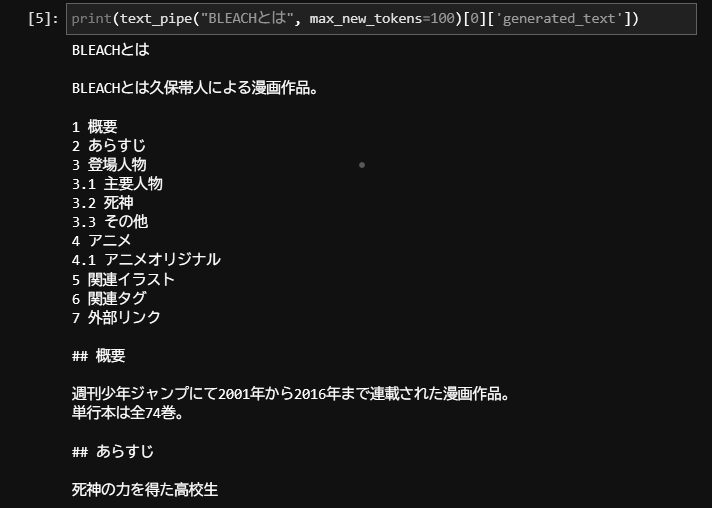
\includegraphics[width=80mm]{../C105Fig/gray/generate.png}
  %\caption{}
  %\label{fig:GoogleColab}
 \end{figure} 

\newpage

文法的にも違和感のない、いい感じの生成結果を得ることができました。目次が挿入されているのはwikipediaか、外部リンクという項目を踏まえるとpixiv大百科あたりの影響を受けている可能性が高いです。事前学習のデータにはCommon CrawlといったWebページのテキストデータが使われているので\footnote{\url{https://llmc.nii.ac.jp/topics/llm-jp-172b/}}、この中にpixiv大百科があってそのテキストを学習したのかもしれません。

WebページのテキストからBLEACHのことを学習済みなら、ポエムも学習済みなのでしょうか? もし学習済みだとすると、fine-tuningに成功した時の結果に対してポエムの微妙な表現の違いを学習しているのか、事前学習時に記憶したポエムを思い出しているだけなのかというように考察が変わってきます。

試しにテキストを与えてみましょう。

\begin{lstlisting}
print(text_pipe("""以下はBLEACHの巻頭のキャッチフレーズです。続きを埋めてください: 
伏して生きるな、""", max_length=30)[0]['generated_text'])
\end{lstlisting}

\begin{figure}[h]
  \centering
  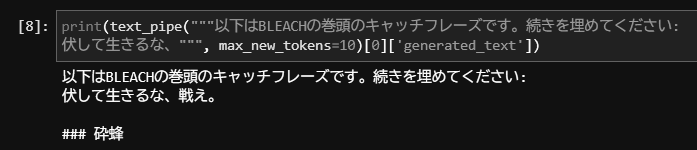
\includegraphics[width=100mm]{../C105Fig/gray/generate_2.png}
  %\caption{}
  %\label{fig:GoogleColab}
 \end{figure} 


だいぶ直球なポエムになりましたね。これをもって学習データにポエムのテキストが含まれていないかという判断は難しいですが、少なくともポエムをはっきり記憶しているわけではなさそうです。

ここまで見てきた通り、日本語能力はそこそこあるがポエム自体の丸暗記まではしていない本モデルがきちんとfine-tuningでポエムの表現の傾向を学習できるか、という点が次章以降のポイントとなります。

\subsection{試しに全パラメータのfine-tuningをしてみる}

PEFT手法を試す前に、本モデルを一般的な手法でfine-tuningすることが難しいことを確認しましょう。まずモデルを読み込んだ段階でのGPUの使用率を``nvidia-smi''コマンドで確認した結果が次の通りです。

\begin{figure}[h]
  \centering
  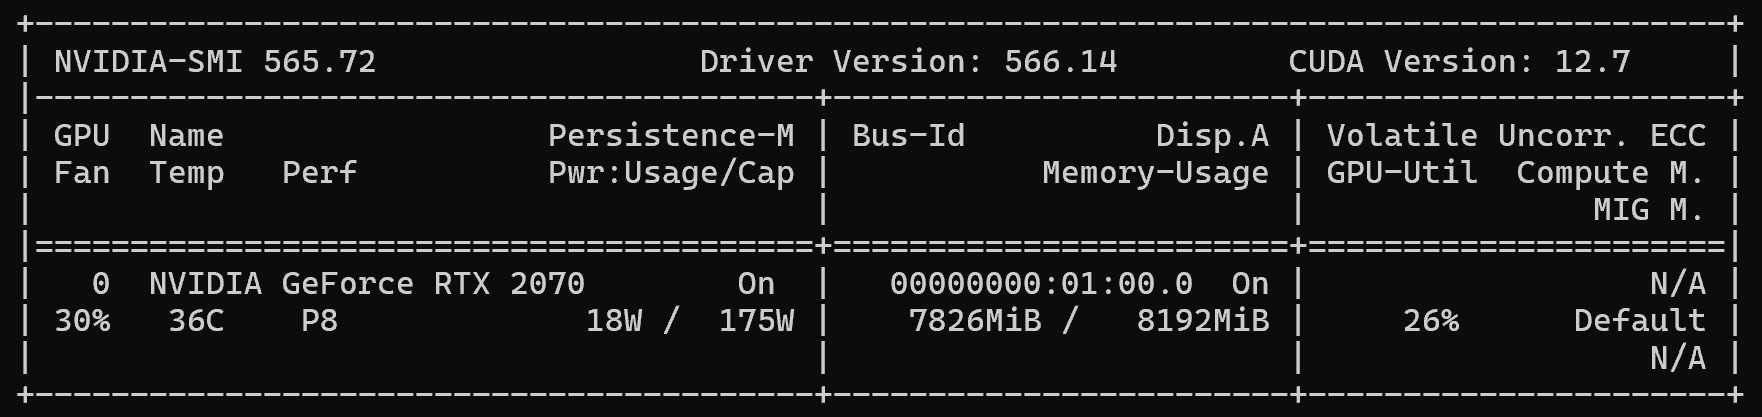
\includegraphics[width=100mm]{../C105Fig/gray/nvidia-smi.png}
  %\caption{}
  %\label{fig:GoogleColab}
 \end{figure} 

GPUにはNVIDIAのGeforce RTX 2070を使っています。メモリサイズは8GBで庶民的な価格のGPUでは一般的ですが、モデルを載せるだけでGPUメモリの大半を使い切っています。32bit floatでパラメータを扱っているのでざっくり1パラメータあたり4Byte、1.8Bパラメータのモデルなので単純計算で7.2GBほど消費する計算です。本GPUは画面描画にも用いているためそちらにもメモリを充てていることを踏まえると、8GBのほとんどを使い切っているのは想定通りといったところです。

推論だけなら何とか動きますが、学習しようとするとこれでは足りません。実際にfine-tuningのコードを実装してみましょう。

まずはモデルを読み込みます。これは``huggingface/transformers''のライブラリを使えば簡単です。

\begin{lstlisting}
from transformers import (
    AutoTokenizer,
    AutoModelForSequenceClassification,
)

tokenizer = AutoTokenizer.from_pretrained(
  "llm-jp/llm-jp-3-1.8b"
)
model = AutoModelForSequenceClassification.from_pretrained(
  "llm-jp/llm-jp-3-1.8b"
)
# 後のTrainerで以下を実行しないと失敗するため入れている設定
model.config.pad_token_id = tokenizer.pad_token_id

\end{lstlisting}

続いて前処理用のクラスを定義します。LLMをはじめとする機械学習モデルは数値計算からなるため、テキストデータはそのままでは扱うことができません。そこでテキストを単語に似たトークンという単位に分割し、それぞれ対応するIDとして数値列にする\textsf{トークナイズ}という処理を行ってからモデルに入力します。それを行うのがtokenizerで、それを動かすためのクラスになります。

\begin{lstlisting}
# テキストのtokenizeを行うための前処理クラス
class TokenizeCollator:
    def __init__(self, tokenizer):
        self.tokenizer = tokenizer

    def __call__(self, examples):
        encoding = self.tokenizer(
            [ex["poem"] for ex in examples],
            padding="longest",
            truncation=True,
            max_length=200,
            return_tensors="pt",
        )
        return {
            "input_ids": encoding["input_ids"],
            "attention_mask": encoding["attention_mask"],
            "labels": torch.tensor([
              ex["labels"] for ex in examples
            ]),
        }

\end{lstlisting}

次はmetricsを計算する関数です。これは学習途中でのvalidデータに対する精度や、学習完了後のtestデータに対する精度を出す関数となっています。``huggingface/evaluate''というライブラリを使って実装しています。

\begin{lstlisting}
import evaluate

roc_auc_evaluate = evaluate.load("roc_auc")
acc_evaluate = evaluate.load("accuracy")
def compute_metrics(eval_pred):
    logits, labels = map(torch.tensor, eval_pred)
    probs = torch.nn.functional.softmax(logits, dim=1)[:, 1]  # label=1の確率
    pred_labels = torch.argmax(logits, dim=1)  # 予測ラベル
    return {
      **roc_auc_evaluate.compute(prediction_scores=probs, references=labels),
      **acc_evaluate.compute(predictions=pred_labels, references=labels),
    }
\end{lstlisting}

必要なものを一通り定義したので学習を実行します。transformersのTrainerを使っています。

\begin{lstlisting}
from transformers import (
    TrainingArguments,
    Trainer,
)

training_args = TrainingArguments(
    output_dir=f"../results/",
    num_train_epochs=10,
    learning_rate=1e-4,
    per_device_train_batch_size=1,
    per_device_eval_batch_size=1,
    weight_decay=1.0,
    evaluation_strategy="epoch",
    logging_strategy="epoch",
    remove_unused_columns=False,
)

trainer = Trainer(
    model=model,
    args=training_args,
    train_dataset=ds["train"],
    eval_dataset=ds["valid"],
    tokenizer=tokenizer,
    data_collator=TokenizeCollator(tokenizer),
    compute_metrics=compute_metrics,
)

trainer.train()
\end{lstlisting}

学習を始めてすぐに、案の定GPUのメモリがあふれてエラーになってしまいました。

\begin{figure}[h]
  \centering
  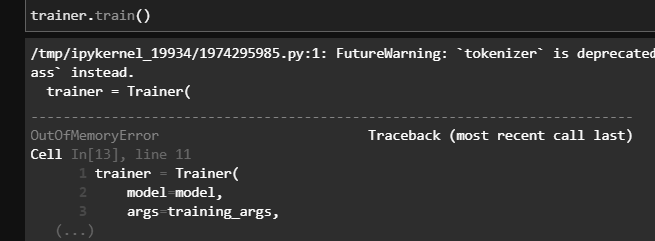
\includegraphics[width=100mm]{../C105Fig/gray/ft_oom.png}
  %\caption{}
  %\label{fig:GoogleColab}
 \end{figure} 

transformersは非常に便利なライブラリで、学習の実装についてはかなりシンプルにできます。ですが計算リソースだけはどうしようもありません。それを解決するため、次章からPEFT手法を一つ一つ見ていきます。

\newpage

\section{低ランク近似により学習するパラメータを減らす}

\subsection{LoRA: 低ランクの差分テンソルを学習}

PEFTの代表格がLow-Rank Adaptation (\textsf{LoRA})です\footnote{E. J. Hu, Y. Shen, P. Wallis, Z. Allen-Zhu, Y. Li, S. Wang, L. Wang, and W. Chen, “Lora: Low-rank adaptation of large language models,” arXiv preprint arXiv:2106.09685, 2021.}。LoRAというと画像生成AIで良くも悪くも取りざたされがちですが、画像に限らずニューラルネットワークのfine-tuning一般に応用可能な技術です。というのもLoRAはテンソルパラメータのfine-tuningを省メモリで行う技術なのですが、ニューラルネットワークは基本的にテンソル演算の繰り返しなのでニューラルネットワークならLoRA適用可能と言って差し支えないためです。

もう少し詳しく書きます。一般のfine-tuningでは事前学習済みモデルのテンソルのパラメータ自体を更新していきます。それに対しLoRAでは元のモデルのパラメータは学習中も固定してしまい、そこからの差分となるテンソルを別途用意してそちらだけを学習します。これだけだとテンソルが増える分無駄にGPUメモリを消費するだけなのですが、追加の工夫として低ランク近似を行います。例えば元のモデルが$1024 \times 1024$のところ、$1024 \times 8$のテンソルと$8 \times 1024$のテンソルの積に近似するといった具合です。この場合パラメータ数は$1024^2 = 1048576$個から$1024 \times 8 \times 2 = 16384$と1/64まで小さくすることができます。学習時に勾配としてメモリが必要になるのは学習対象のパラメータ分のみなので、1.8Bモデルならもともと勾配に7.2GB必要とするところ、LoRAにより約110MBまで圧縮できます。モーメントに必要なメモリも同様です。

\newpage

\begin{figure}[h]
  \centering
  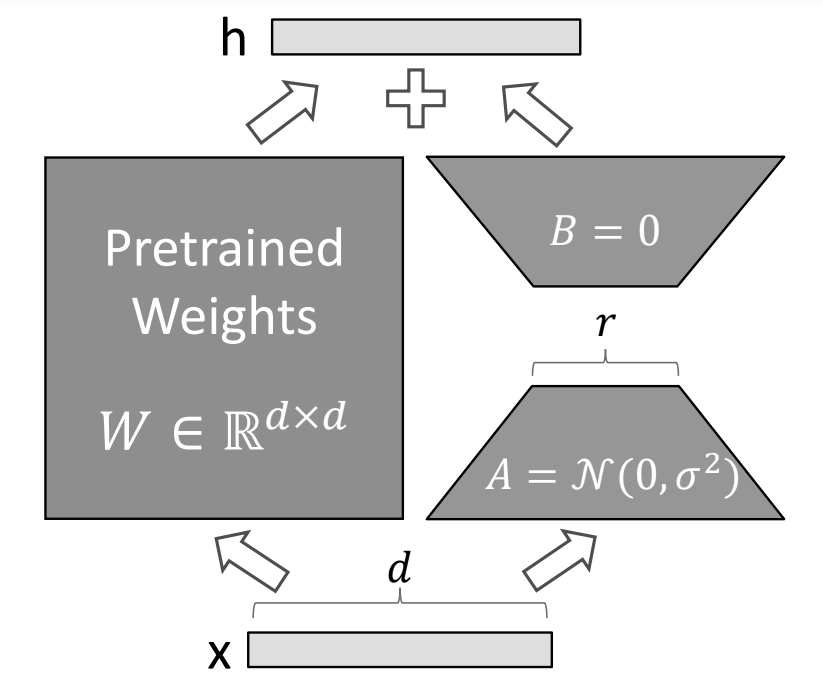
\includegraphics[width=80mm]{../C105Fig/gray/lora_image.png}
  %\caption{}
  %\label{fig:GoogleColab}
 \end{figure} 

PEFTの他手法と比べたLoRAの利点としては、学習後は差分テンソルを元のテンソルと足し合わせて一つのモデルにマージすることで、推論時の計算量を元のモデルと同じにすることができるという点です。後述する他の手法ではモデルの中に追加の計算処理を入れて、その処理におけるパラメータを学習するパターンが多いです。そのケースでは推論時にも追加の計算処理を実行する必要があるため、どうしても元のモデルより計算量は増えてしまいます。それを回避できる点でLoRAは魅力的です。

またLoRAの低ランク近似は、元のモデルの知識がfine-tuningによって失われる\textsf{破滅的忘却}という現象を回避する良い正則化になっているという議論もあります\footnote{D. Biderman, J. Portes, J. J. G. Ortiz, M. Paul, P. Greengard, C. Jennings, D. King, S. Havens, V. Chiley, J. Frankle, C. Blakeney, and J. P. Cunningham, “LoRA Learns Less and Forgets Less,” arXiv preprint. arXiv:2405.09673 [cs.LG] (2024).}。これが事実であれば、省メモリなだけでなくLLMの知識を引き出し精度を出すfine-tuning手法としても理にかなっているということになります。

説明はこれくらいにして、実際に実行してみましょう! PEFT手法は``huggingface/peft''というライブラリにまとめられていて、LoRAを含む様々な手法を統一された書き方で簡単に実装することができます。

\begin{lstlisting}
from peft import LoraConfig, TaskType
from peft.peft_model import PeftModelForSequenceClassification

# PeftModelForSequenceClassificationにバグがあるため
# 関数の差し替えをしている
class PatchedPeftModelForSequenceClassification(
  PeftModelForSequenceClassification):
    def add_adapter(
      self,
      adapter_name,
      peft_config, 
      low_cpu_mem_usage=False):
        super().add_adapter(adapter_name, peft_config)

peft_config = LoraConfig(
  task_type=TaskType.SEQ_CLS,
  r=1,
)

peft_model = PatchedPeftModelForSequenceClassification(
  model, peft_config)
\end{lstlisting}

たったこれだけの実装で元のモデルの重みを固定し、LoRAの低ランク差分テンソルと連携させることができます。実際に学習するパラメータがどれくらい減ったか見てみましょう。

\begin{lstlisting}
peft_model.print_trainable_parameters()
# 出力: trainable params: 200,704 || all params: 1,663,870,976 || trainable%: 0.0121
\end{lstlisting}

全パラメータが16.6億\footnote{パラメータ数が1.8Bよりも小さいのは、もとはText GenerationモデルをClassificationモデルとして読み込むことにより、生成のために特別に必要なテンソルが破棄されていることなどが理由だと思われます。}に対して、学習するパラメータは20万と、実に0.01%程度まで減らせています。今回の設定では低ランク近似のランクを1にまで圧縮しているので、学習対象のパラメータも4桁も下げることができているのです。これにより、学習中に必要な勾配などのために保持しておくメモリ容量は誤差程度となるため、最低限のGPUメモリ消費で学習を動かせます。

それでは実際に学習させてみましょう。学習スクリプトは2章3節のスクリプトのTrainerに渡すmodelという変数をpeft\_modelに置き換えるだけです。

\begin{figure}[h]
  \centering
  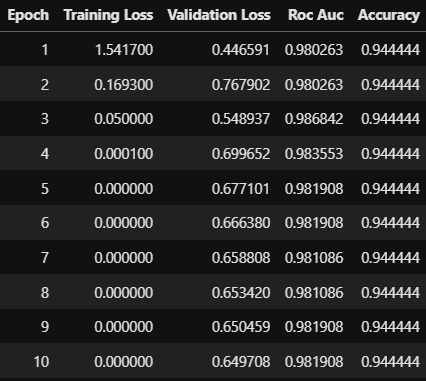
\includegraphics[width=60mm]{../C105Fig/gray/lora_train.png}
  %\caption{}
  %\label{fig:GoogleColab}
 \end{figure} 


まず、メモリのエラーを起こさずにきちんと学習が進行しました。これだけでもPEFT手法を使う意義があります。また学習に伴うvalidデータへの精度を見ると1 epochでAUC 0.98を超え、Accuracyは0.944に収束しています。またtestデータへのAccuracyは0.963でこちらも良好です。

2章1節で触れた通り、今回使うデータセットはPEFT手法ごとの性能を比較するにはサイズが小さすぎるため、指標の値からLoRAの精度面における優位性について論じることはできません。しかし少なくとも意味のある学習ができているとは言ってよいでしょう。

\subsection{AdaLoRA: LoRAのランクをいい感じに決める}

さて、LoRAで効率よくLLMのfine-tuningができることが確認できたのは良いのですが、賢い人は次のように考えました。「LLMの全てのテンソルで同じランクの近似を行っているが、テンソルごとにランクを変えた方が良いのではないか」と。

LLMはTransformerブロックと呼ばれるSelf Attentionと全結合を組み合わせたブロックを何層も重ねています。その層は深さに応じて役割が異なると言われており、それは浅いブロックでは単語同士の関係や短いフレーズなどの特徴を抽出する一方、深いほど広い文脈や抽象的な概念の情報を処理する、といった具合です。実際にこれを問題提起した\textsf{AdaLoRA}という手法の提案論文\footnote{Q. Zhang, M. Chen, A. Bukharin, P. He, Y. Cheng, W. Chen, and  T. Zhao, “Adaptive budget allocation for parameter-efficient fine-tuning,” arXiv preprint arXiv:2303.10512, 2023. }\footnote{AdaLoRAは`Adaptive Low-Rank Adaptation'の略とのこと。Adaptionがかぶっている……。}では、LLMの層別にLoRAを適用すると層が深いテンソルへのLoRAモデルの方がfine-tuning後の精度が上がることを確認しています。

\newpage

\begin{figure}[h]
  \centering
  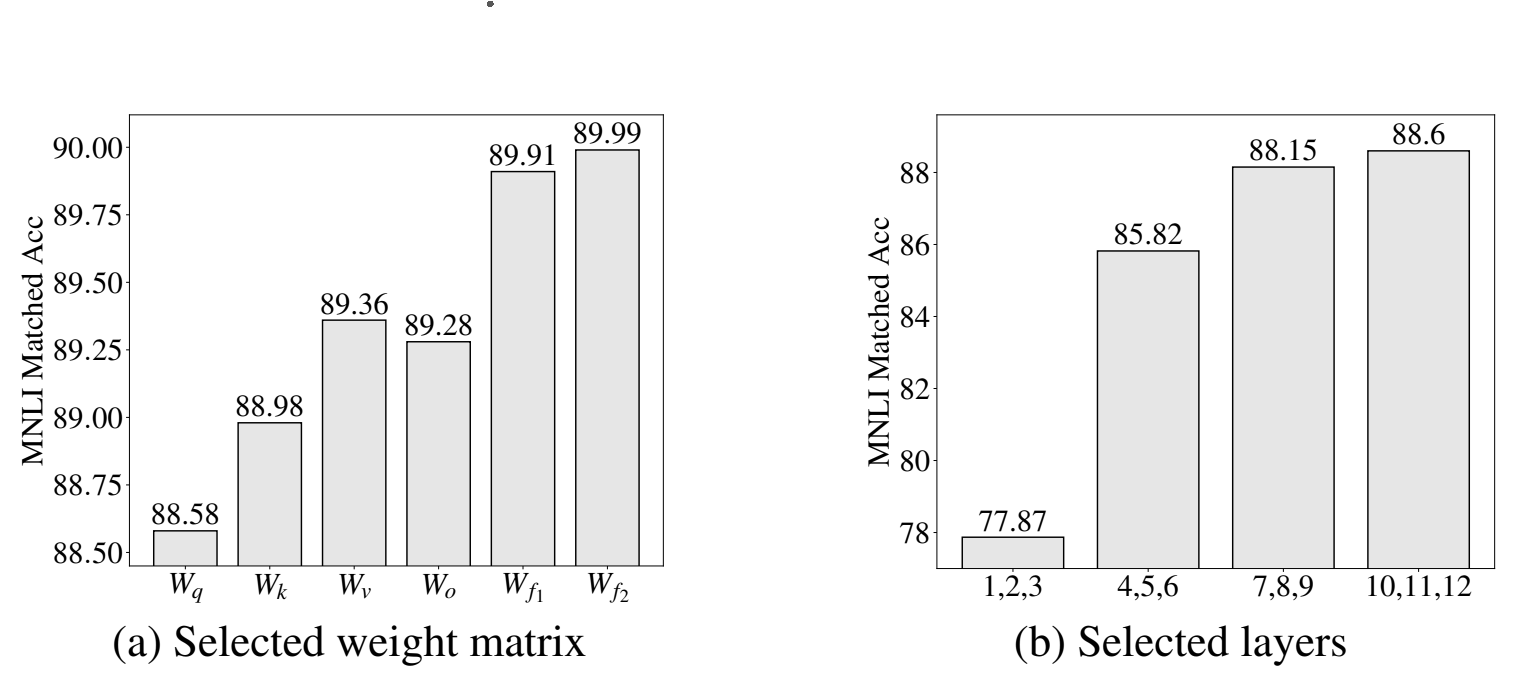
\includegraphics[width=100mm]{../C105Fig/gray/adalora_layers.png}
  %\caption{}
  %\label{fig:GoogleColab}
 \end{figure} 

であればレイヤーごとに異なるランクのテンソルを学習しよう! ……となるのですが、たくさんあるレイヤーそれぞれランクを調整すると組み合わせ爆発して探索が大変になってしまいます。そこでAdaLoRAでは、学習中に層ごとの重要度を計測し、その重要度に応じてランクを割り当てるというテクニックが開発・導入されました。テクニックの詳細は原著をご参照いただければと思いますが、ざっくり説明すると、

\begin{enumerate}
  \item 低ランク近似を特異値分解の形に変換したうえで
  \item 学習が進むごとに、中央の対角テンソルの各値およびそれに紐づく左右のテンソルの要素に対する損失関数の勾配から重要度を計算
  \item それが小さいものは精度への影響が小さい要素ということで対角テンソルの要素を0にしてしまう
\end{enumerate}

という流れにより、最初は全体的に高めにランクを割り当てたところから間引いていくことで最終的に重要度に合わせたランクに落とし込んでいきます。

と、長々書きましたが、このような細かいロジックを知らなくてもとりあえず動かすことはできます。先ほどのLoRAConfigをAdaLoRAConfigに書き換えるだけです。

\begin{lstlisting}
from peft import AdaLoraConfig, TaskType
peft_config = AdaLoraConfig(
    task_type=TaskType.SEQ_CLS,
    init_r=2,
    target_r=0.5,
)
\end{lstlisting}

最初は1テンソルあたりランク2からスタートして、最終的には1テンソルあたりランク0.5まで間引くような設定を書きました。実際には対角テンソルの非ゼロの要素が0個のテンソル、1個のテンソル、2個のテンソルが重要度に応じて決定されるという挙動を期待しています。

学習した結果は次の通りです。


\begin{figure}[h]
  \centering
  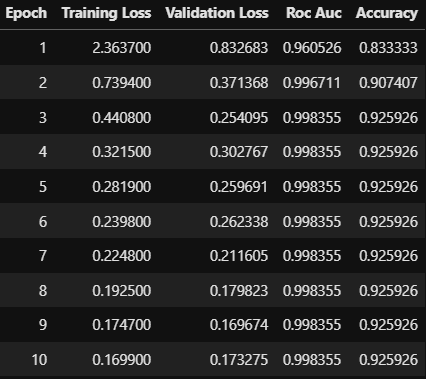
\includegraphics[width=60mm]{../C105Fig/gray/adalora_train.png}
  %\caption{}
  %\label{fig:GoogleColab}
 \end{figure} 

LoRAに比べると少し収束までステップを要していますが、最終的にはAccuracy 0.926に落ち着きました。testデータへのAccuracyは0.944となり、良い精度が出ています。

LoRAの派生手法はAdaLoRA以外にも数多く存在します。一部はより高精度を求め、一部はより高速・省メモリになるように発展させ、``huggingface/peft''ライブラリで利用できるものも数多くあります。このように派生が数多くあることがLoRAという手法の優秀さを物語っているといえるでしょう。

\newpage

\section{入力プロンプトを最適化する}

\subsection{Prompt tuning: 仮想プロンプトを学習}

LLMと言えばプロンプトエンジニアリング、すなわちLLMの出力を見ながらプロンプトを調整することで目的のタスクを解かせるような使い方が定番です。この枠組みをfine-tuningに応用したのが仮想プロンプト系の手法で、\textsf{Prompt tuning}もその一つです\footnote{B. Lester, R. Al-Rfou, and N. Constant, “The power of scale for parameter-efficient prompt tuning,” arXiv preprint arXiv:2104.08691, 2021}。

Prompt tuningの趣旨はプロンプトエンジニアリングと比較するとわかりやすいです。プロンプトエンジニアリングでは、人が様々にプロンプトを入力します。例えば以下のようなものです。

\begin{lstlisting}
次に挙げるポエムがBLEACHのものかCOMIC LOのものか分類してください: {ポエム}
\end{lstlisting}

この入力に対してLLMはまず『次に挙げるポエムがBLEACHのものかCOMIC LOのものか分類してください:』というプロンプトをまずトークン分割したうえで、Embedding層を通してトークンごとに埋め込みベクトルに変換し横につなげます。結果として、もしプロンプトが20個のトークンに分割された場合、出力は(20, ベクトル次元)のshapeを持つテンソルになります。ポエムも同様にトークン分割・埋め込みベクトルに変換し、つなげてテンソルとします。得られたテンソル同士も横につなげて一つのテンソルとしたのち、多層Transformerでトークン間の関係を解釈していきます。

Prompt tuningでは実際のプロンプトのテンソルの代わりに、例えば(20, ベクトル次元)の学習可能なテンソルを用意し、ポエムに対応するテンソルの横につなげます。ここで20という数字はハイパーパラメータです。学習時にはこの仮想プロンプトの埋め込みテンソルに対して勾配逆伝播を行いパラメータを調整していきます。%またプロンプトエンジニアリングと異なり、出力層を置き換えることで分類結果のテキスト生成ではなく各クラスの確率を直接出力する分類モデルに変換することができ、より分類タスクに最適化することができます。


\begin{figure}[h]
  \centering
  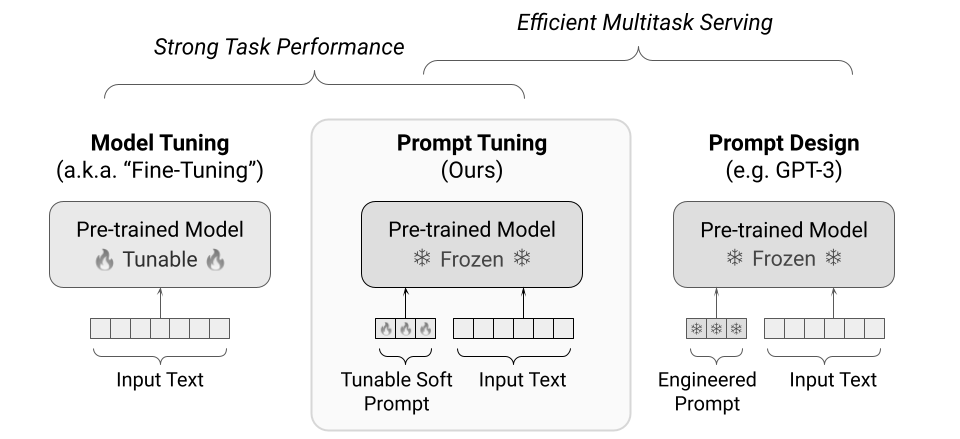
\includegraphics[width=100mm]{../C105Fig/gray/prompttuning_image.png}
  % \caption{}
  %\label{fig:GoogleColab}
 \end{figure} 

 
 \rightline{\footnote{図の出典: https://research.google/blog/
 
 guiding-frozen-language-models-with-learned-soft-prompts/}}

通常のプロンプトエンジニアリングがトークンを離散的に選びながら調整する一方、Prompt tuningでは連続的に値をとれるパラメータを勾配法で調整することから、前者をハードプロンプト・後者をソフトプロンプトと呼ぶことがあります。

Prompt tuningの趣旨を説明したところで実際に動かしてみましょう。前章の低ランク近似とは全く異なる手法ですが、``huggingface/peft''ライブラリでは全く同じ書き方でOKです。

\begin{lstlisting}
from peft import PromptTuningConfig, TaskType

peft_config = PromptTuningConfig(
    task_type=TaskType.SEQ_CLS,
    num_virtual_tokens=10,
)
\end{lstlisting}

この設定で学習した結果が以下の通りです。


\begin{figure}[h]
  \centering
  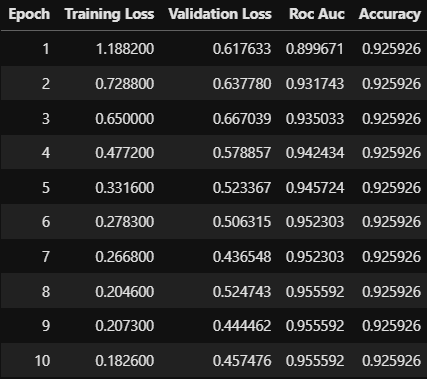
\includegraphics[width=60mm]{../C105Fig/gray/prompttuning_train.png}
  % \caption{}
  %\label{fig:GoogleColab}
 \end{figure} 


前章のLoRA・AdaLoRAとは異なりTraining Lossからして少し不安定です。一応validデータのAccuracyはそこそこ出ているものの、testデータへのAccuracyは0.815と比較的小さめに出てしまいました。

LoRAと異なりPrompt tuningは入力という勾配逆伝播の終点部分のみを学習する\footnote{一応クラスごとのlogitsを計算する最後の全結合層も学習しますが。}ため、勾配を伝える間にノイズが乗りやすく学習が難しいのかもしれません。とはいえデータが少ないですから、手法の優劣についてここで論じるのは早計であることは改めて書いておきます。

\subsection{P-Tuning: 仮想プロンプトの埋め込みにニューラルネットワークを挟む}

ソフトプロンプトを勾配法で学習するのが素朴には難しいということは知られており、仮想プロンプトの埋め込みを直接ポエムのテンソルと結合するのではなく、ニューラルネットワークを通してから結合する\textsf{P-Tuning}という手法も提唱されています\footnote{X. Liu, Y. Zheng, Z. Du, M. Ding, Y. Qian, Z. Yang, and J. Tang, “GPT understands, Too,” arXiv preprint arXiv:2103.10385, 2021.}\footnote{P-TuningのPはPromptという意味だと思うのですが、論文を斜め読みした限りでは特に言及はありませんでした。}。具体的には以下の通りで、トークン埋め込みにあたるテンソル$h_{0:m}$をi番目で分割し、ニューラルネットワークの学習可能なレイヤーの1つであるLong Short Term Memory(LSTM)とMulti Layer Perceptron(MLP)に通しています。

$$
h_i = \mathrm{MLP} \left( [\overrightarrow{h}_i : \overleftarrow{h}_i] \right) \\
= \mathrm{MLP} \left( [\mathrm{LSTM}(h_{0:i}) : \mathrm{LSTM}(h_{i:m})] \right)
$$

これにより学習結果にどのような影響があるのでしょうか? 設定は以下の通りです。

\begin{lstlisting}
from peft import PromptEncoderConfig, TaskType
  
peft_config = PromptEncoderConfig(
    task_type=TaskType.SEQ_CLS,
    num_virtual_tokens=10,
)
\end{lstlisting}

そして学習した結果が次の通りです。

\newpage

\begin{figure}[h]
  \centering
  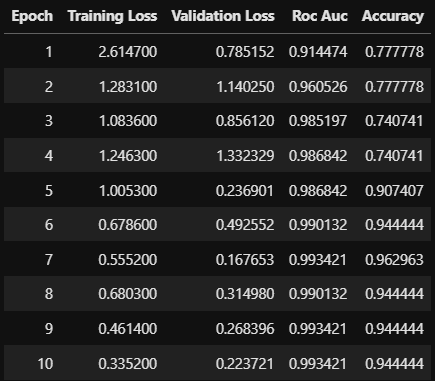
\includegraphics[width=60mm]{../C105Fig/gray/ptuning_train.png}
  % \caption{}
  %\label{fig:GoogleColab}
 \end{figure} 

valid AUCなどは少しPrompt tuningよりも良くなっています。testデータへのAccuracyは0.852とこちらも少し改善しました。が、データ数を踏まえると誤差の範囲とも言えるかもしれません。

なおあたかもP-TuningをPrompt tuningの発展手法のように書いていますが、実際にはP-Tuningの提案論文はPrompt tuningよりも1カ月早く世に出ています。明確な優劣もついておらずタスク・データセットごとに相性があるという報告もあり\footnote{X. Liu, K. Ji, Y. Fu, W. L. Tam, Z. Du, Z. Yang, and J. Tang, “P-tuning v2: Prompt tuning can be comparable to fine-tuning universally across scales and tasks,” arXiv preprint arXiv:2110.07602, 2021.}、どちらがより良い手法かについては実験的に探索するのが望ましいでしょう。

\newpage

\section{内部に追加のアダプターを導入する}

\subsection{$\rm{(IA)^3}$: 各層の出力をベクトルで補正する}

低ランクの差分テンソル・仮想プロンプトに続く第3のPEFT手法が内部的な出力を変換するアダプターを挟むという手法です。その中でも$\rm{(IA)^3}$はLoRAよりさらにfine-tuningするパラメータ数が小さい手法として知られています\footnote{H. Liu, D. Tam, M. Muqeeth, J. Mohta, T. Huang, M. Bansal, and C. A. Raffel, “Few-shot parameter-efficient fine-tuning is better and cheaper than in-context learning,” Advances in Neural Information Processing Systems, vol. 35, pp. 1950–1965, 2022.}\footnote{$\rm{(IA)^3}$は`Infused Adapter by Inhibiting and Amplifying Inner Activations'の略とのこと。}。

$\rm{(IA)^3}$ではTransformerブロックにおけるテンソルの一部(一般的にはSelf AttentionのKey, Valueとそれに続くFeed Forward Network(FFN)の1層目)の出力に対して学習可能なベクトルを定義し、各トークンに対応するベクトルに対して要素ごとに積を取ることでその出力を補正します。


\begin{figure}[h]
  \centering
  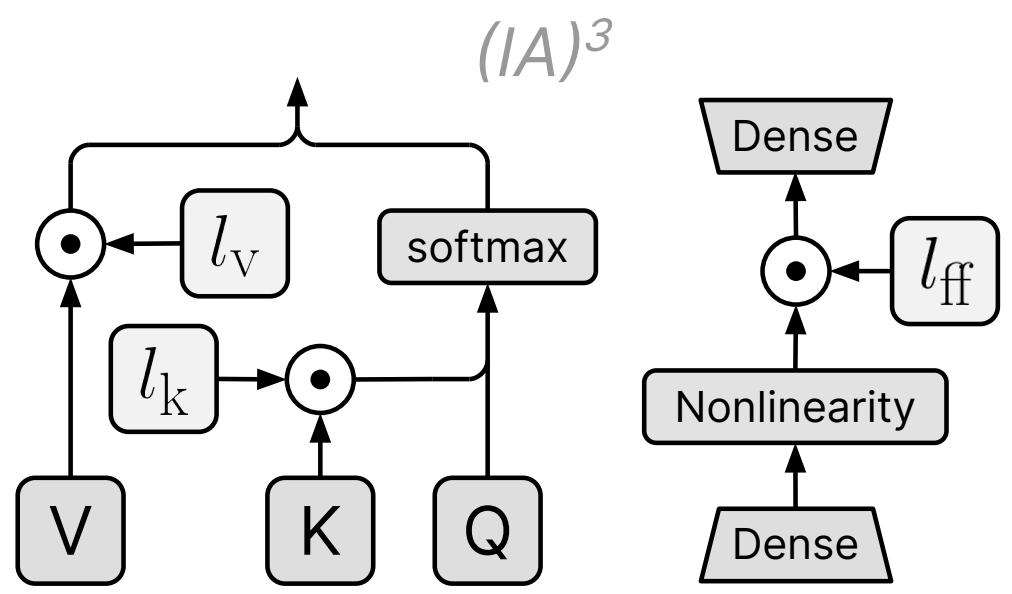
\includegraphics[width=80mm]{../C105Fig/gray/ia3_image.png}
  % \caption{}
  %\label{fig:GoogleColab}
 \end{figure} 

LoRAの場合はざっくり(トークンごとの埋め込み次元 $\times$ 低ランク近似のランク数 $\times$ 2 $\times$ 近似するテンソルの数 $\times$ Transformerブロックの数)分のパラメータを学習することになりますが\footnote{厳密にはFFNの1層目の埋め込み次元のみ異なる点を考慮する必要があります。}、$\rm{(IA)^3}$だと(トークンごとの埋め込み次元 $\times$ 学習可能なベクトルで補正するテンソルの数 $\times$ Transformerブロックの数)分のパラメータを学習するだけで済みます。ただLoRAでもかなり学習するパラメータ数を減らせることからGPUメモリの節約効果は絶対値的には大差なく、学習速度もほとんど変わらないことが多いです。

なお$\rm{(IA)^3}$はLoRAと同様に学習後にはベクトルと各テンソルをかけ合わせてマージすることで、推論は元のモデルと同じ計算量で済みます。LoRAのランクのようなハイパーパラメータもないため、$\rm{(IA)^3}$で十分に精度が出る場合にはこちらを選ぶのも良いでしょう。

それでは動かしてみましょう。$\rm{(IA)^3}$はハイパーパラメータもほとんどなく設定もかなりシンプルです。

\begin{lstlisting}
from peft import IA3Config, TaskType
 
peft_config = IA3Config(task_type=TaskType.SEQ_CLS)
\end{lstlisting}


\newpage

\begin{figure}[h]
  \centering
  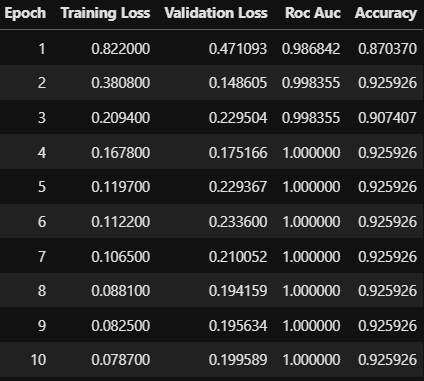
\includegraphics[width=60mm]{../C105Fig/gray/ia3_train.png}
  % \caption{}
  %\label{fig:GoogleColab}
 \end{figure} 

 
学習は比較的速く進み、validデータへの精度も安定しています。testデータのAccuracyは0.926とこちらも良好でした。


\subsection{LLaMa-Adapter: AttentionのKeyとValueを外部からも与える}

Adapterを入れる手法としてもう一つ、LLaMa-Adapterを紹介しておきましょう\footnote{R. Zhang, J. Han, A. Zhou, X. Hu, S. Yan, P. Lu, H. Li, P. Gao, and Y. Qiao, “Llama-adapter: Efficient fine-tuning of language models with zero-init attention,” arXiv preprint arXiv:2303.16199, 2023.}。

\newpage

LLaMa-AdapterはTransformerブロックのSelf Attentionの前方に、仮想的な埋め込みにあたるテンソルから計算したAttentionのKeyとValueをつなげる手法です。学習可能なテンソルを前方につなげるという意味では仮想プロンプトを学習する手法に近いですが、Transformerブロックのうち出力層に近い数ブロックを対象にする点が違いとなります。主なハイパーパラメータとしては仮想的なプロンプトのトークン数と出力から何ブロックまでさかのぼって適用するかの2つがあります。


\begin{figure}[h]
  \centering
  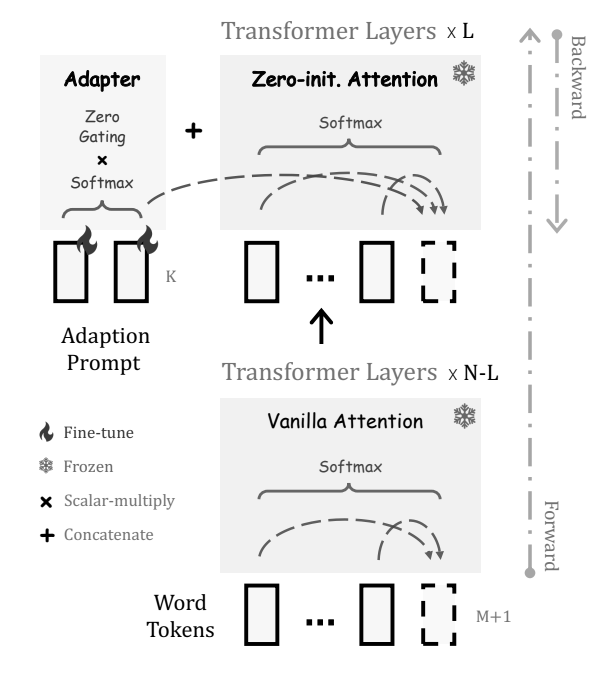
\includegraphics[width=70mm]{../C105Fig/gray/llama_adapter_image.png}
  % \caption{}
  %\label{fig:GoogleColab}
 \end{figure} 

 \newpage

LLaMa-Adapterの特徴としては、仮想的なプロンプトの代わりに画像などを埋め込んで渡しても良いという点です。これにより、画像を入力しつつ「これに写っている標識はどういう意味ですか?」と自然文で尋ねるなどのマルチモーダルなタスクに答えることができます。学習時には画像をテキストと同じ意味空間に落とし込むような学習をすることで、LLMのパラメータは固定したまま画像入力を受け取ることができるようになります\footnote{察しのいい人は気づいたかもしれませんが、同じ理屈でPrompt TuningやP-Tuningもマルチモーダル化することは可能で、そういった研究もあります。}。


\begin{figure}[h]
  \centering
  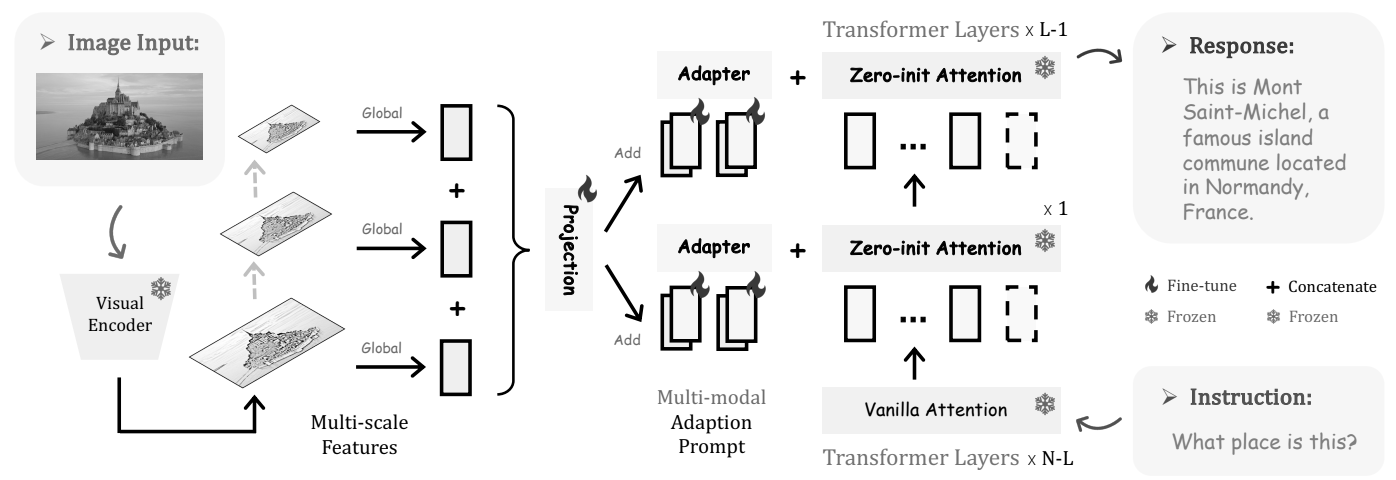
\includegraphics[width=100mm]{../C105Fig/gray/llama_adapter_image2.png}
  % \caption{}
  %\label{fig:GoogleColab}
 \end{figure} 

LLaMa-Adapterはその名前のとおりLLaMaと呼ばれるMeta社が公開するLLMのネットワーク構造に依存した手法で、他のネットワーク構造のLLMに適用するのは難しい場合があります。しかし本書で利用するllm-jp/llm-jp-3-1.8bモデルはLLaMaと同じ構造を採用しており、LLaMa-Adapterも利用可能です。さっそく試してみましょう。

\begin{lstlisting}
from peft import AdaptionPromptConfig, TaskType

peft_config = AdaptionPromptConfig(
    task_type=TaskType.SEQ_CLS,
    adapter_layers=8,
    adapter_len=10,
)
\end{lstlisting}



\begin{figure}[h]
  \centering
  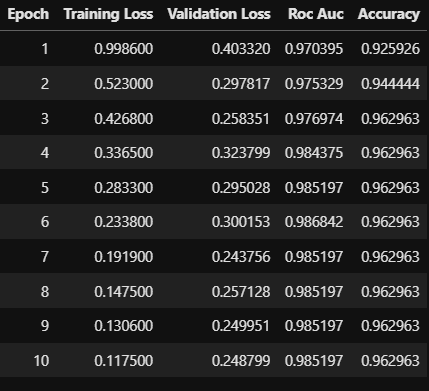
\includegraphics[width=60mm]{../C105Fig/gray/llama_adapter_train.png}
  % \caption{}
  %\label{fig:GoogleColab}
 \end{figure} 

学習は非常に安定して進みました。仮想プロンプト系の手法と異なり出力層に近い部分の勾配のみが考慮されることが安定に寄与している……かもしれません。testデータへのAccuracyは0.963でこちらも良好でした。

なおLLaMa-Adapterについては$\rm{(IA)^3}$などとは異なりレイヤーをマージして推論時には元のモデルと同じ推論時間というわけにはいきません。ただし計算量が増えるのはAttentionの部分だけですので、仮想トークン数が同じなら仮想プロンプト系の手法よりは計算量は抑えられると考えられます。

\newpage

\section{おわりに}

以上が代表的なPEFT手法になります。いずれも興味深い工夫で数少ないパラメータからモデルの性能を引き出していましたね。

今や様々な企業・機関がLLMを公開しており、その性能も日進月歩です。せっかく自由にパラメータをいじれる公開LLMをプロンプトエンジニアリングだけで扱うのはもったいないことで、目的に合わせたラベル付きデータセットでfine-tuningすることでその可能性を引き出すことができます。学習するハードウェアの確保が難しいとなった場合には、ぜひ本書の内容を思い出してみてください。

誰でもプロンプトでAIを活用できるAI民主化の時代になっても、精度を突き詰めるシーンで機械学習エンジニアの役割がなくなることはありません。AIに使われず、AIを使いこなす気概で次の時代を切り拓いていきましょう。

\newpage

\thispagestyle{empty} 

\textcolor{white}{.}
\vspace{\baselineskip}
\vspace{\baselineskip}
\vspace{\baselineskip}
\vspace{\baselineskip}
\vspace{\baselineskip}
\vspace{\baselineskip}
\vspace{\baselineskip}
\vspace{\baselineskip}
\vspace{\baselineskip}
\vspace{\baselineskip}
\vspace{\baselineskip}
\vspace{\baselineskip}
\vspace{\baselineskip}
\vspace{\baselineskip}
\vspace{\baselineskip}
\vspace{\baselineskip}
\vspace{\baselineskip}
\begin{screen}

実践PEFT ~ご家庭のGPUでLLM fine-tuning~

\begin{tabbing}
  0000000 \= 000 \= \kill
  著者 \> お椀の底の玉 \\
  発行日 \> 2024/12/30 (初版) \\
  発行元 \> ゆるふわ数理研究所 \\
  X ID \> @yurufuwasuuri \\
  印刷所 \> ちょ古っ都製本工房
\end{tabbing}

\end{screen}

\vspace{\baselineskip}
% 本書で使用したスプレッドシートは

% % \url{https://docs.google.com/spreadsheets/d/1-R35DSPx9mZpWCph}

% % \url{WSuliG8pkzbRLOUb9ySijESiDlc/edit?usp=sharing}

% で閲覧が可能です。


\end{document}
\